\documentclass[aspectratio=169,t]{beamer}
\usepackage[utf8]{inputenc}
\usepackage[T1]{fontenc}
\usepackage[english]{babel}
\usepackage{hyperref}
\usepackage{tikz}

\usepackage{graphicx}
\usepackage{epstopdf}
\usepackage{multirow}

\usepackage{psfrag}
\usepackage{pgfplots}
\usepackage{framed}
\usepackage{xcolor}
\usepackage{booktabs}
\usepackage{caption}
\usepackage{epstopdf}
\usepackage{amsmath}
\usepackage{tabularx}
\usepackage[]{bookmark}
%\usepackage[3D]{movie15}
%\usepackage{media9}
\usepackage[binary-units,abbreviations]{siunitx}
\usepackage[textfont=normalsize, labelfont=normalsize, justification=centering]{subcaption}
\usepackage{marvosym}
\usepackage{calc}
\usepackage{color, colortbl}
\usepackage[]{svg} 
\usepackage[]{trfsigns} 
\usepackage[nomessages]{fp}
\usepackage[]{csquotes}\MakeOuterQuote{"}
\usepackage{tabto}
\selectcolormodel{rgb}

\makeatletter
\def\beamer@calltheme#1#2#3{\def\beamer@themelist{#2}
	\@for\beamer@themename:=\beamer@themelist\do
	{\usepackage[{#1}]{\beamer@themelocation/#3\beamer@themename}}}
\def\usefolder#1{\def\beamer@themelocation{#1}}
\def\beamer@themelocation{}
\usefolder{theme}

\usetikzlibrary{matrix,
	decorations.pathreplacing,
	calc,
	positioning,
	external,
	3d,
	shapes,
	arrows,
	pgfplots.statistics}
\pgfplotsset{compat=1.16}
\tikzstyle{faunode}=[rounded corners, draw=faublue, fill=faublue!10,  align=center, inner sep=0.3cm, line width=0.4mm]
\tikzstyle{fauellipseFixedWidth}=[ellipse, draw=faublue, fill=faublue!10,  align=center, inner sep=0.3cm, line width=0.4mm, minimum width=3cm]
\tikzstyle{fauellipse}=[ellipse, draw=faublue, fill=faublue!10,  align=center, inner sep=0.3cm, line width=0.4mm]
\tikzstyle{fauarrow}=[draw=faublue,->, line width=0.4mm]
\tikzstyle{fauline}=[draw=faublue, line width=0.4mm]


\usepackage[backend=bibtex,sorting=none,doi=true,style=phys]{biblatex}
%\usepackage[]{biblatex}
\bibliography{./references}

% Themes:
%  - fau:          FAU theme
%  - fau-tf:       TechFak FAU theme
%  - fau-tf-lme:   TechFak LME FAU theme
%  - fau-tf-aibe:  TechFak AIBE FAU theme
%
% Options:
%  - image:        Cover image on title page
%  - plain:        Plain title page
%  - longtitle:    Title page layout for long title
% \usetheme[longtitle]{fau-tf-lme}
\usetheme[longtitle]{fau-tf-aibe}

% END of THEME SETTINGS
% --------------------------------------------------------------------------------------------------------------------------------------------------------------------------

\sisetup{
exponent-product =\ensuremath{{\,\cdot\,}}
}

% Enable semi-transparent animation preview
\setbeamercovered{transparent}
\setbeamertemplate{blocks}[rounded]
\captionsetup{labelformat=empty,labelsep=none, labelfont=normalsize, justification=centering}


\newcommand\Wider[2][1.0cm]{%
\makebox[\linewidth][c]{%
  \begin{minipage}{\dimexpr\textwidth+#1\relax}
  \raggedright#2
  \end{minipage}%
  }%
}


\let\origitem\item
\renewcommand{\item}{\normalfont\origitem}
\newcommand{\bluefat}[1]{\textcolor{faublue}{\textbf{#1}}}
\newcommand{\bolditem}{\normalfont\origitem\bfseries}
\newcommand{\question}{{\bf Question: }}
\newcommand{\answer}{{\bf Answer: }}
\newcommand{\myExample}{{\bf Example }}
\newcommand{\real}{\mbox{${\mathbb R}$}}
\definecolor{defColor}{rgb}{0.8,0.87,0.97}
\definecolor{defColorT}{rgb}{0,0,0}
\definecolor{defColorF}{rgb}{1,1,1}
\newenvironment{myDefinition}{%
	\def\FrameCommand{\fboxsep=\FrameSep{} \fcolorbox{defColorF}{defColor}}%
	\color{defColorT}\MakeFramed{\FrameRestore{}}}%
{\endMakeFramed}

% Title page
\title[Medical Engineering II]{Medical Engineering - Imaging Systems}

\author{Prof.\ Dr. Bernhard Kainz \and Prof.\ Dr. Florian Knoll}
\date{SS 2024}
\institute{IDEA Lab and Computational Imaging Lab at Dept. AIBE}

\newcommand{\password}{\texttt{mt2\_ss22}}


\AtBeginSection[]{
	{
		\setbeamertemplate{footline}{}
		\begin{frame}[noframenumbering]{\insertsubtitle}
			 \tableofcontents[currentsection]
		\end{frame} 
	}
}
\AtBeginSubsection[]{
	{

		\setbeamertemplate{footline}{}
		\begin{frame}[noframenumbering]{\insertsubtitle}
			 \tableofcontents[currentsection, currentsubsection]
		\end{frame} 
	}
}


\usepackage{bm}
\usepackage[]{colorwav} 
\usepackage{etoolbox}
\newcommand{\abs}[1]{\ensuremath{\big\vert #1\big\vert}}

%\addtobeamertemplate{frametitle}{\vskip-1.2cm}{}

\subtitle{Optical Coherence Tomography}

\AtBeginSection[]{
    {
        \setbeamertemplate{footline}{}
        \begin{frame}[noframenumbering]{\insertsubtitle}
            \large \tableofcontents[currentsection]
        \end{frame} 
    }
}
\AtBeginSubsection[]{
    {

        \setbeamertemplate{footline}{}
        \begin{frame}[noframenumbering]{\insertsubtitle}
            \large \tableofcontents[currentsection, currentsubsection]
        \end{frame} 
    }
}

\begin{document}
% Title page
\title[OCT]{Optical Coherence Tomography}

\frame[plain,c]{\titlepage} % plain-Option deaktiviert Kopf- und Fusszeile
\section{Introduction}

%\begin{frame}[c]{Outline}
%\begin{itemize}
%\setlength\itemsep{0.3cm}
%\item Introduction
%\item Working principle of OCT
%\begin{itemize}
%\item Light as a wave
%\item Interference
%\item Coherence length
%\item OCT Setup
%\end{itemize}
%\item Applications
%\begin{itemize}
%\item Retinal imaging
%\item Cardiovascular imaging
%\end{itemize}
%\item Take home messages
%\item Further reading
%\end{itemize}
%\end{frame}



\begin{frame}
    \frametitle{What is OCT?}
    \begin{columns}[T]
        \column{0.48\textwidth}

        \begin{itemize}
            \item OCT = Optical Coherence Tomography
            \item Optical tomographic technique
            \item Non-invasive
            \item Mircometer resolution
            \item Major application: Clinical retinal imaging
        \end{itemize}
        \column{0.49\textwidth}
        \bigskip
        %\hspace{-0.3 cm}
        \begin{figure}
            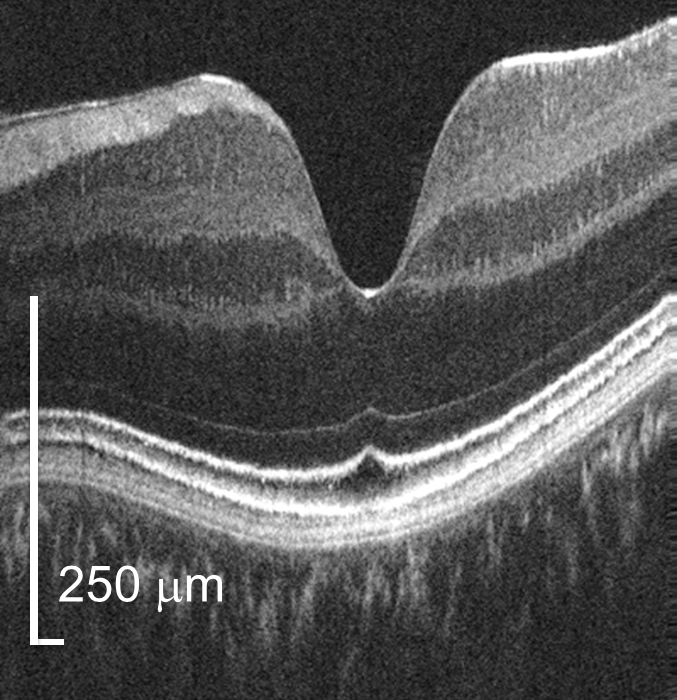
\includegraphics[height=0.7\textheight]{figures/OCTSample.png}
            \caption{2D-OCT Image of Human Macula}
        \end{figure}
    \end{columns}
\end{frame}


\begin{frame}
    \frametitle{History of OCT}

    \begin{itemize}
        \item Concept invented by multiple groups in parallel
              \begin{itemize}
                  \item A. F. Fercher (1990)
                  \item Naohiro Tanno (1990)
                  \item D. Huang (1991)
              \end{itemize}
        \item Major initial publication: Huang, D; Swanson, EA; Lin, CP; Schuman, JS; Stinson, WG; Chang, W; Hee, MR; Flotte, T et al. (1991). ``Optical coherence tomography''. Science 254 (5035): 1178–81.

        \item Since then:
              \begin{itemize}
                  \item 10 times better resolution
                  \item 1000 times higher speed
                  \item At the same time!
              \end{itemize}
    \end{itemize}
\end{frame}


\begin{frame}
    \frametitle{Advantages of OCT}

    \begin{columns}[T]
        \column{0.48\textwidth}

        \begin{itemize}
            \item Pure optical method
            \item No ionizing radiation – enabling safe use
            \item In situ imaging of tissue microstructure with a resolution approaching that of histology, but without the need for tissue excision and processing
            \item Live sub-surface images at near-microscopic resolution
            \item Instant imaging of tissue morphology
        \end{itemize}

        \column{0.49\textwidth}
        %	\bigskip

        \begin{figure}
            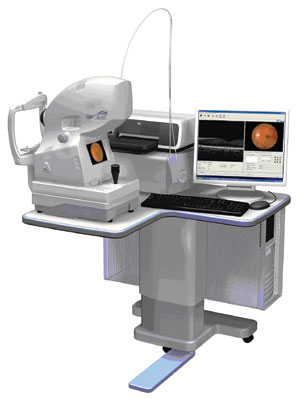
\includegraphics[height=0.7\textheight]{figures/OCTSystem.png}
            \caption{OCT System}
        \end{figure}
    \end{columns}

\end{frame}



\begin{frame}
    \frametitle{OCT Compared to other modalities}

    \begin{figure}
        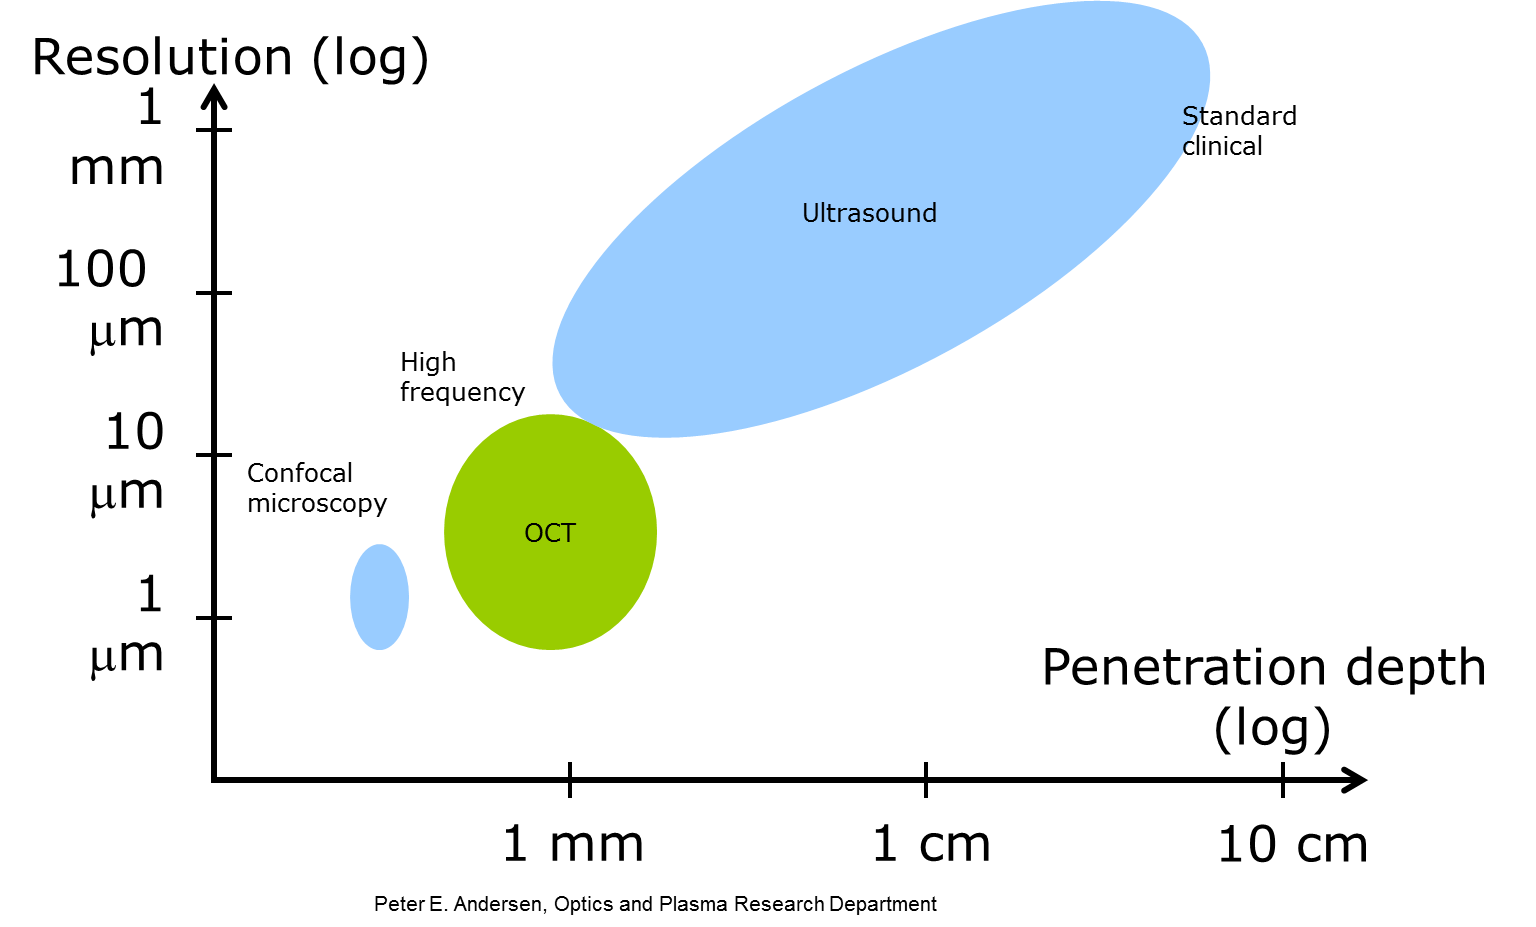
\includegraphics[height=0.8\textheight]{figures/ResolutionComparison.png}
        %\caption{O}
    \end{figure}

\end{frame}


\section{Working Principle of OCT}

\subsection{High Level Overview}%
\label{sub:high_level_overview}


\begin{frame}[c]{High level overview}

    \textbf{\color{faublue}{Optical Coherence Tomography:}}
    \vspace{0.3cm}
    \begin{itemize}
        \setlength\itemsep{0.3cm}
        \item Uses a beam of light to acquire information about tissue
        \item Beam is focused onto tissue
        \item Uses low-coherence interferometry (LCI) to obtain the depth and strength of reflections along the beam
        \item Scans the beam to construct 2D and 3D images from the 1D depth profiles obtained with LCI
    \end{itemize}


\end{frame}


\subsection{Light as a Wave}%
\label{sub:light_as_a_wave}


\begin{frame}
    \frametitle{Light as a wave}


    \begin{itemize}
        \item Light is electromagnetic radiation and has wave nature
        \item Propagation speed: $c=\SI{3e8}{m/s}$ (in vacuum)
        \item Very high frequency: $f=\SI{4e14}{Hz}$ (red light)
        \item Wavelength: $\lambda = \frac{c}{f}$ (approx. $\SI{700}{nm}$ for red light)
    \end{itemize}

    \begin{figure}
        \centering{}
        \scalebox{0.9}{\renewcommand*{\do}[1]{
  \storeRGBofWavelength{\Rval}{\Gval}{\Bval}{#1}
  \definecolor{wl#1}{rgb}{\Rval, \Gval, \Bval}
}
\newdimen\XCoord
\newdimen\YCoord
\newcommand*{\ExtractCoordinate}[1]{\path (#1); \pgfgetlastxy{\XCoord}{\YCoord};}%
\docsvlist{380,400,450,500,550,600,650,700,750,780}

\pgfdeclarehorizontalshading{spectrum}{1.5cm}{
  color(0cm)=(wl380);
  color({0.2cm})=(wl400); color(0.7cm)=(wl450);
  color(1.2cm)=(wl500); color(1.7cm)=(wl550);
  color(2.2cm)=(wl600); color(2.7cm)=(wl650);
  color(3.2cm)=(wl700); color(3.7cm)=(wl750);
  color(4cm)=(wl780)
}

\begin{tikzpicture}


  \node (spectrum) [inner sep=0pt] {\pgfuseshading{spectrum}};
  \node (visible_box) [above=1.1cm of spectrum.north,draw=black!50, minimum height=1.5cm, fill=yellow!60] {\rotatebox{90}{Visible}};

  \node (uv_box) [left=0cm of visible_box.west,draw=black!50, minimum height=1.5cm, minimum width=0.6cm] {UV};
  \node (xray_box) [left=0cm of uv_box.west,draw=black!50, minimum height=1.5cm, minimum width=1.7cm] {X-rays};
  \node (gamma_box) [left=0cm of xray_box.west,draw=black!50, minimum height=1.5cm] {Gamma rays};

  \node (ir_box) [right=0cm of visible_box.east,draw=black!50, minimum height=1.5cm] {Infrared};
  \node (micro_box) [right=0cm of ir_box.east,draw=black!50, minimum height=1.5cm] {Microwaves};
  \node (radio_box) [right=0cm of micro_box.east,draw=black!50, minimum height=1.5cm] {Radio frequency};

  \node (visible) [above=0.0cm of spectrum.north]  {\footnotesize Visible spectrum};
  \node (purple) [below=0.1cm of spectrum.south west]  {\SI{400}{nm}};
  \node (red) [below=0.1cm of spectrum.south east]  {\SI{750}{nm}};

  %\node (left_wave) [above=0.2cm of xray_box.north west]  {\tiny $10^{-11}$};
  \ExtractCoordinate{xray_box.north west}
  \foreach \x in {-0,...,7}
  {
    \FPeval{\result}{round(2*\x-11,0)}
    \node (right_wave) [] at ( 1.2cm*\x + \XCoord, 3.7cm )  {\color{black!80}{\scriptsize $10^{\result}$\,m}};
  \node (foo) [] at ( 1.2cm*\x+\XCoord, \YCoord ) {};
  \path[draw=black!30, line width=0.4mm] (right_wave.south) -- (foo.center) node[midway, above right] {};

  }
  \node (wavelength) [above left=0.3cm and 0.1cm of gamma_box.north west, anchor=west, inner sep= 0]  {\scriptsize \color{black!80}{Wavelength:}};
  

  %\node (right_wave) [above=0.2cm of xray_box.north west]  {\footnotesize $10^{-3}$};

  \path[draw=black!50] (spectrum.north east) -- (visible_box.south east) node[midway, above right] {};
  \path[draw=black!50] (spectrum.north west) -- (visible_box.south west) node[midway, above right] {};
\end{tikzpicture}
}
        %\includegraphics[height=0.45\textheight]{figures/VisibleSpectrum.png}
        %\caption{The visible spectrum. Source: \url{http://www.chem.ufl.edu/~itl/4411/lectures/lec_10.html}}
    \end{figure}

\end{frame}


\begin{frame}
    \frametitle{Wave equation}

    \begin{columns}[t, onlytextwidth]
        \begin{column}{0.5\textwidth}
            \begin{itemize}
                \item For a monochromatic (single color) wave in 1D:
                \item $E(t,x) = A \cdot \cos\left( 2 \pi \left(f \cdot t + \frac{x}{\lambda} \right) + \varphi \right)$
                \item $A$ : Amplitude
                \item $t$ : Time
                \item $x$ : 1D spatial coordinate
                \item $\varphi$: Initial phase
                \item Argument to cosine: (Overall) phase
                \item The disturbance depends on time AND space!
                \item Example equation: $ 1 \cdot \cos(10 \cdot t + 1.0 \cdot x + 0) $
            \end{itemize}
        \end{column}\begin{column}{0.5\textwidth}
            \begin{figure}
                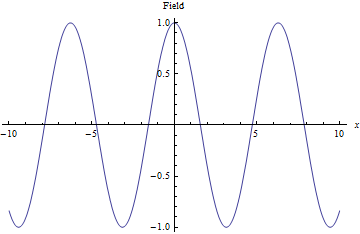
\includegraphics[width=\textwidth]{figures/Wave_t0.png}
                \caption{Plot of a Wave at fixed time $t=0$}
            \end{figure}
        \end{column}
    \end{columns}



\end{frame}


\begin{frame}
    \frametitle{Wave equation (2)}

    \begin{itemize}
        \item As time progresses, the hills and valleys of the wave travel
    \end{itemize}

    \begin{figure}
        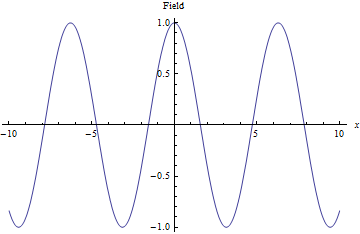
\includegraphics[height=0.65\textheight]{figures/Wave_t0.png}
        \caption{Plot of a wave at fixed time $t=0$}
    \end{figure}

\end{frame}


\begin{frame}
    \frametitle{Wave equation (3)}

    \begin{itemize}
        \item As time progresses, the hills and valleys of the wave travel
    \end{itemize}

    \begin{figure}
        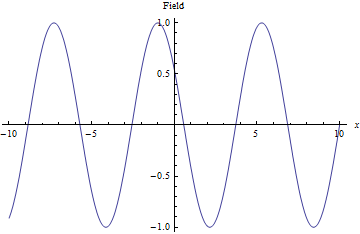
\includegraphics[height=0.65\textheight]{figures/Wave_t01.png}
        \caption{Plot of a wave at fixed time $t=0.1$}
    \end{figure}

\end{frame}


\begin{frame}
    \frametitle{Wave equation (4)}

    \begin{itemize}
        \item As time progresses, the hills and valleys of the wave travel
    \end{itemize}

    \begin{figure}
        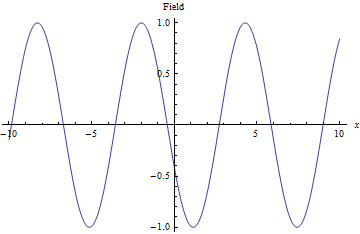
\includegraphics[height=0.65\textheight]{figures/Wave_t02.png}
        \caption{Plot of a wave at fixed time $t=0.2$}
    \end{figure}

\end{frame}

\begin{frame}
    \frametitle{Light detection}

    \begin{itemize}
        \item If light is a wave, why don't we see the hills and valleys?
              \begin{itemize}
                  \setlength\itemsep{0.1cm}
                  \item The frequency $f$ is too high for our eyes (or any electronic detector) to see the oscillations (recall: $f=\SI{4e14}{Hz}$ (red light) )
                  \item Also: Detectors don't detect the field $E(t,x)$ but the square of it, called \emph{intensity} $E(t,x)^2$
              \end{itemize}
        \item What is detected: Time average of intensity
              %\begin{itemize}
              \begin{equation} I(t,x) = \langle E(t,x)^2 \rangle = \frac{1}{T} \int_t^{t+T}{  E(t',x)^2 } dt'\end{equation}
              %\end{itemize}
        \item $T \gg \frac{1}{f}$
        \item For a monochromatic wave: $E(t,x) = A \cdot \cos\left( 2 \pi \left(f \cdot t + \frac{x}{\lambda} \right) \right)$
        \item $I = \frac{1}{2} A^2$
    \end{itemize}

\end{frame}

\subsection{Interference}


\begin{frame}[c]{Superposition Principle}

    \begin{itemize}
        \setlength\itemsep{0.3cm}
        \item For multiple waves $E_1(x,t)$, $E_2(x,t)$, ... $E_n(x,t)$
        \item The net field is the sum of the individual fields
              \begin{equation}
                  E_{overall}(x,t) = \sum_i{ E_i(x,t) }
              \end{equation}
        \item This is what leads to interference
        \item \textbf{However:} Not detecting field but time averaged intensity

    \end{itemize}

\end{frame}



\begin{frame}
    \frametitle{Interferometer}

    \begin{itemize}
        %\item The light source emits a wave $E(x,t)$
        \item<2-> The half transparent mirror splits the light into two parts
        \item<3-> The two parts travel two distances $x_1$ and $x_2$, reflect at the respective mirror and reach the central mirror again where the fields add
        \item<4-> The time averaged intensity of the combined field is detected by a detector
    \end{itemize}

    \begin{figure}
        %\includegraphics[height=0.65\textheight]{figures/Interferometer.png}
        \def\svgwidth{0.5\textwidth}
        \input{interferometer.pdf_tex}
        \caption{(Michelson) Interferometer}
    \end{figure}

\end{frame}

\begin{frame}[t]{Interferometer (2)}
    What happens when $x_1$ is varied?

    \begin{center}
        \def\svgwidth{0.5\textwidth}
        \input{interferometer_move.pdf_tex}
    \end{center}


\end{frame}

\begin{frame}{Interferometer (3)}

    \begin{itemize}
        \item<1-> The first wave has to travel $2x_1$ while the second travels $2x_2$ before getting back to the mirror
        \item<2-> If $x_1 \neq x_2$ a \emph{phase difference} is introduced between the two waves

    \end{itemize}
    \begin{center}
        \scriptsize
        \def\svgwidth{0.5\textwidth}
        \input{interferometer_move.pdf_tex}
    \end{center}


\end{frame}

\begin{frame}{Interferometer (4)}

    For a fixed frequency/wavelength $\lambda$:
    \vspace{0.4cm}
    \begin{itemize}
        \item Phase change by path length $\delta x$:
              \begin{equation}
                  2 \pi \frac{ \delta x}{\lambda}
              \end{equation}
        \item Phase difference through path length difference:
              \begin{equation}
                  \varphi(x_1-x_2) = 2 \pi   \frac{ x_1 - x_2 }{\lambda}
              \end{equation}

    \end{itemize}
    %\begin{center}
    %\scriptsize
    %\def\svgwidth{0.4\textwidth}
    %\input{interferometer_move.pdf_tex}
    %\end{center}


\end{frame}


\begin{frame}
    \frametitle{Interferometer (5)}


    \begin{itemize}
        \item Monochromatic light source:


    \end{itemize}
    \begin{align}
        E_{combined}(x,t) & =\cos\left( 2 \pi \left(f \cdot t + \frac{x}{\lambda} \right) \right) + \cos\left(2 \pi \left( f \cdot t + \frac{x}{\lambda} \right) + 2\varphi\left(x_1-x_2\right)\right) \\
                          & = 2 \cos\left( \varphi\left(x_1-x_2\right)\right) \cos\left( 2 \pi\left( f \cdot t + \frac{x}{\lambda} \right) + \varphi\left(x_1-x_2\right)\right)
    \end{align}

    \begin{itemize}
        \item Right part: fastly oscillating, averages out
        \item Left part: only depends on phase difference, will not average out over time
        \item Leads to stable interference
        \item $I = \cos\left(\varphi\left(x_1-x_2\right)\right)^2$
    \end{itemize}


\end{frame}


\begin{frame}
    \frametitle{Interference Pattern for Monochromatic light}
    \begin{itemize}
        \item Stable recurring interference pattern, regardless of how large the difference between mirror positions is
    \end{itemize}

    \begin{figure}
        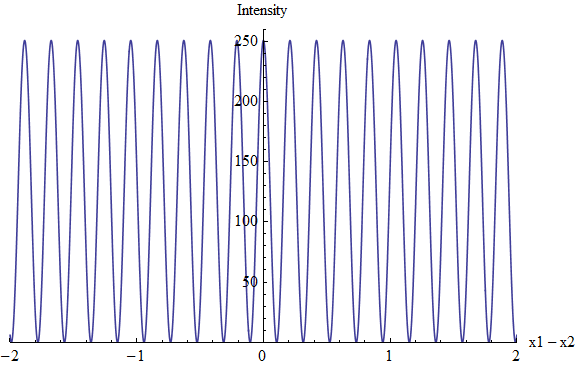
\includegraphics[height=0.65\textheight]{figures/Interference0.png}
        \caption{Interference Pattern for monochromatic light}
    \end{figure}

\end{frame}


\begin{frame}
    \frametitle{Increasing the bandwidth}
    \begin{itemize}
        \item Instead of only a single frequency wave (think: red light) we can also have a light source with many different colors (think: white light)

              \begin{equation}
                  E(t,x) = \sum_i{A_i \cdot \cos\left(f_i \cdot t + \frac{x}{\lambda_i} + \varphi_i\right)}
              \end{equation}
        \item The wider the spread between the different frequencies $f_i$ the higher the bandwidth of the source, the whiter the light
    \end{itemize}

\end{frame}


\begin{frame}
    \frametitle{Multiple Wavelengths, but little Bandwidth}
    %\begin{itemize}
    %\item Stable recurring interference pattern , regardless of how large the difference between mirror positions is
    %\end{itemize}

    \begin{figure}
        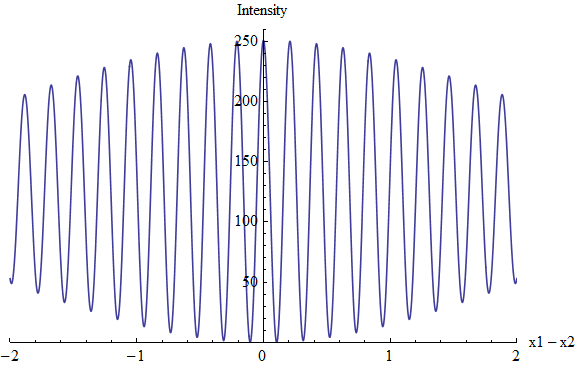
\includegraphics[height=0.65\textheight]{figures/Interference1.png}
        %	\caption{Interference Pattern for monochromatic light}
    \end{figure}

\end{frame}


\begin{frame}
    \frametitle{Doubling the Bandwidth}
    %\begin{itemize}
    %\item Stable recurring interference pattern , regardless of how large the difference between mirror positions is
    %\end{itemize}

    \begin{figure}
        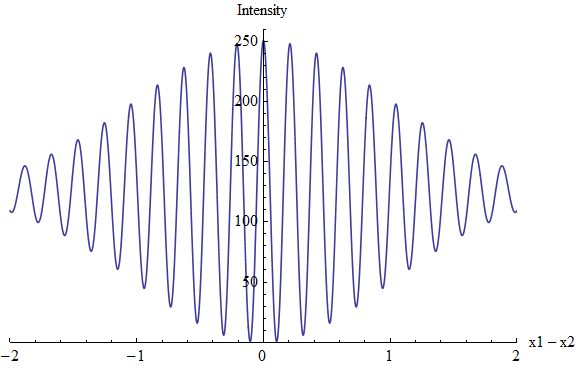
\includegraphics[height=0.65\textheight]{figures/Interference2.png}
        %	\caption{Interference Pattern for monochromatic light}
    \end{figure}

\end{frame}



\begin{frame}
    \frametitle{Doubling Again}
    %\begin{itemize}
    %\item Stable recurring interference pattern , regardless of how large the difference between mirror positions is
    %\end{itemize}

    \begin{figure}
        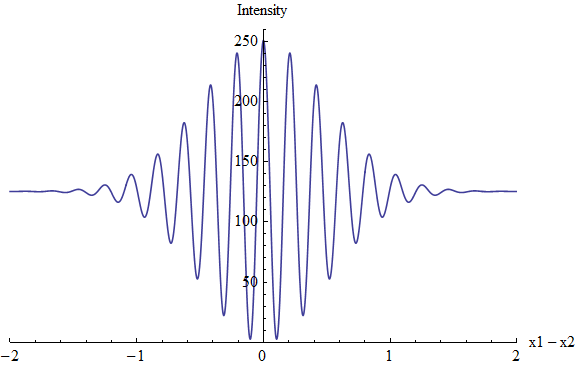
\includegraphics[height=0.65\textheight]{figures/Interference3.png}
        %	\caption{Interference Pattern for monochromatic light}
    \end{figure}

\end{frame}


\begin{frame}
    \frametitle{And Again}
    %\begin{itemize}
    %\item Stable recurring interference pattern , regardless of how large the difference between mirror positions is
    %\end{itemize}

    \begin{figure}
        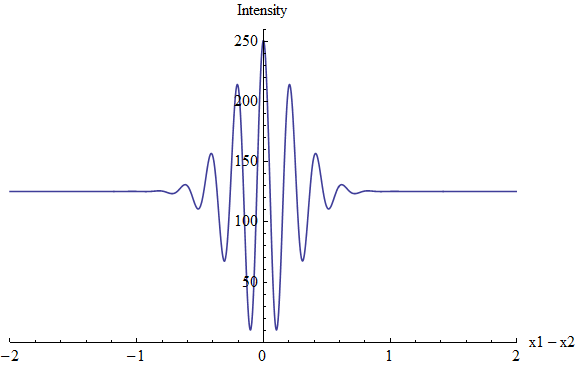
\includegraphics[height=0.65\textheight]{figures/Interference4.png}
        %	\caption{Interference Pattern for monochromatic light}
    \end{figure}

\end{frame}


\begin{frame}[c]{Coherence length}
    \begin{itemize}
        \setlength\itemsep{0.3cm}
        \item<1-> \bluefat{Observation:} The higher the bandwidth of the source, the sooner interference vanishes
        \item<2-> \bluefat{Coherence length:} Maximum difference in mirror positions for which we still see interference
              \vspace{0.3cm}
              \begin{itemize}
                  \setlength\itemsep{0.2cm}
                  \item<3-> For \bluefat{monochromatic light} the coherence length is infinite
                  \item<4-> The more \bluefat{different frequencies} the shorter the coherence length
                  \item<5-> For a light source with short coherence length we will only see oscillations if the paths are closely matched!
              \end{itemize}
    \end{itemize}

\end{frame}


\begin{frame}
    \frametitle{Low Coherence Interferometry}
    \begin{itemize}
        \item Suppose an interferometer as before but with two mirrors
        \item Also: We don't know the distance $x_3$
    \end{itemize}
    \begin{figure}
        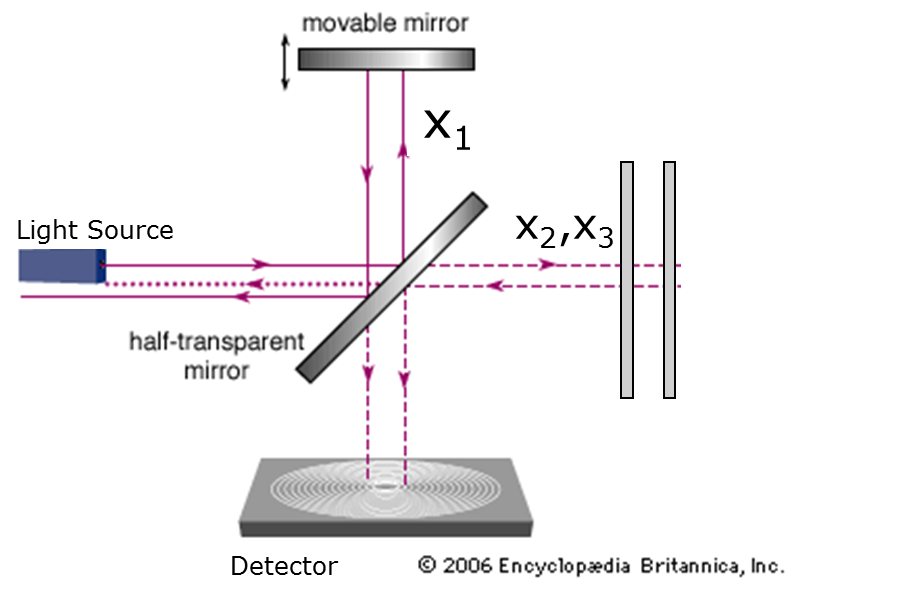
\includegraphics[height=0.65\textheight]{figures/DoubleMirror.png}

    \end{figure}

\end{frame}



\begin{frame}
    \frametitle{Low Coherence Interferometry (2)}
    \begin{itemize}
        \item Idea: Scan the mirror (vary $x_1$) and observe the signal
        \item Will see one interference pattern appear if $x1$ well matched to $x_2$ and one if $x1$ is well matched to $x_3$
    \end{itemize}
    \begin{figure}
        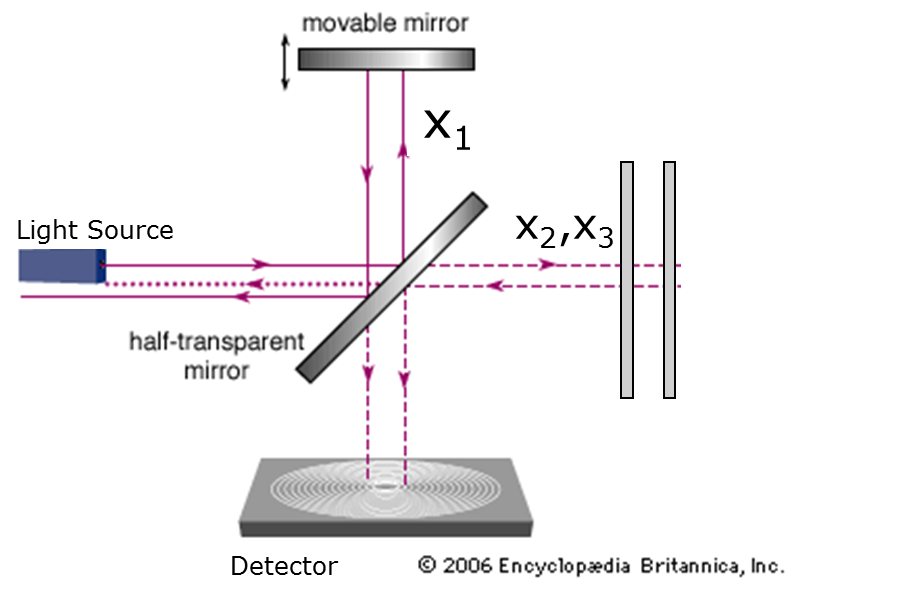
\includegraphics[height=0.65\textheight]{figures/DoubleMirror.png}

    \end{figure}

\end{frame}


\begin{frame}
    \frametitle{Two Mirrors}
    \begin{itemize}
        \item What's the distance between $x_2$ and $x_3$?
    \end{itemize}
    \begin{figure}
        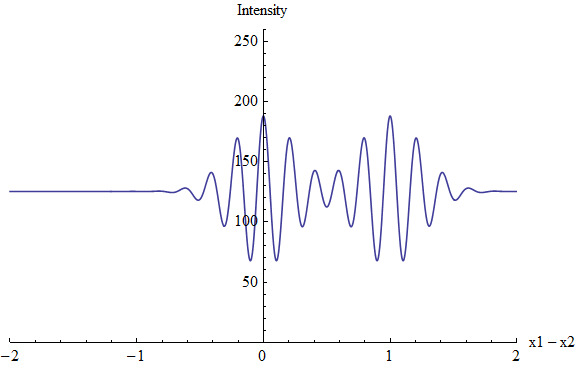
\includegraphics[height=0.65\textheight]{figures/DoubleInterference1.png}
        %	\caption{Interference Pattern for monochromatic light}
    \end{figure}

\end{frame}


\begin{frame}
    \frametitle{Two Mirrors, Again Doubling Bandwidth}
    \begin{itemize}
        \item Better separation interference patterns, better \emph{resolution}
    \end{itemize}
    \begin{figure}
        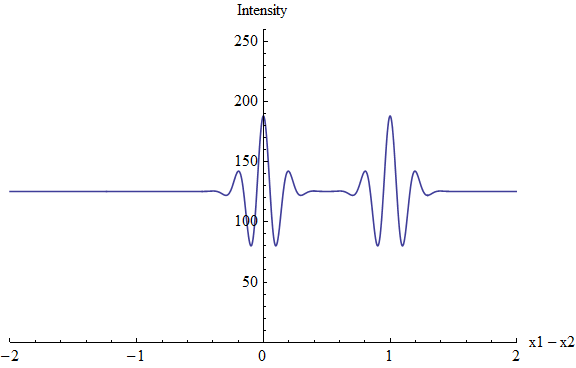
\includegraphics[height=0.65\textheight]{figures/DoubleInterference2.png}
        %	\caption{Interference Pattern for monochromatic light}
    \end{figure}

\end{frame}



\begin{frame}
    \frametitle{From LCI to (Time-Domain) OCT}
    \begin{itemize}
        \item<2-> Instead of mirrors, place a sample
        \item<3-> \emph{Scan} the movable mirror to acquire one axial scan (A-Scan)
        \item<4-> \emph{Scan} the beam that probes the sample using a scanning system (B-Scan)
    \end{itemize}

    \centering{}
    \scalebox{0.75}{%
        \begin{columns}[b, onlytextwidth]
            \begin{column}{0.5\textwidth}
                \begin{figure}[]
                    \centering
                    \def\svgwidth{\textwidth}
                    \only<1>{
                        \input{td_oct_with_mirror.pdf_tex}
                        \caption{Setup for Low Coherence Interferometry}
                    }
                    \only<2->{
                        \input{td_oct.pdf_tex}
                        \caption{Setup for Time-Domain OCT}
                    }
                \end{figure}
            \end{column}\begin{column}{0.5\textwidth}
                \begin{figure}[]
                    \centering
                    \only<-3>{
                        \visible<3>{
                            \def\svgwidth{0.8\textwidth}
                            \input{raster_scan_a.pdf_tex}
                            \caption{A-Scan}
                        }
                    }
                    \only<4>{
                        \def\svgwidth{0.8\textwidth}
                        \input{raster_scan_2d.pdf_tex}
                        \caption{B-Scan (2D)}
                    }
                    \only<5>{
                        \def\svgwidth{0.8\textwidth}
                        \input{raster_scan.pdf_tex}
                        \caption{B-Scan (3D)}
                    }
                \end{figure}
            \end{column}
        \end{columns}%
    }
    %\begin{figure}
    %\includegraphics[height=0.65\textheight]{figures/HuangSystem.pdf}
    %%	\caption{Interference Pattern for monochromatic light}
    %\end{figure}

\end{frame}

\begin{frame}
    \frametitle{Nowadays: Fourier Domain OCT}
    \vspace{-0.3cm}
    \begin{itemize}
        \item Fixed mirror position, spectrometer instead of detector
        \item No mechanical moving parts, instantaneous A-Scan Info
        \item Enables much higher speed, better sensitivity
        \item A-Scan $\Rightarrow$ Fourier Transform (Spectrum)
    \end{itemize}
    %\begin{figure}
    %\includegraphics[height=0.55\textheight]{figures/SpectralSchematic.pdf}
    %%	\caption{Interference Pattern for monochromatic light}
    %\end{figure}
    \only<1>{

        \begin{figure}[]
            \centering
            \def\svgwidth{0.45\textwidth}
            \input{td_oct_with_fixed_reference.pdf_tex}
            \vspace{-0.3cm}
            \caption{Setup for Fourier OCT with fixed reference}
        \end{figure}
    }

    \only<2>{
        \begin{columns}[b, onlytextwidth]
            \begin{column}{0.5\textwidth}
                \begin{figure}[]
                    \centering
                    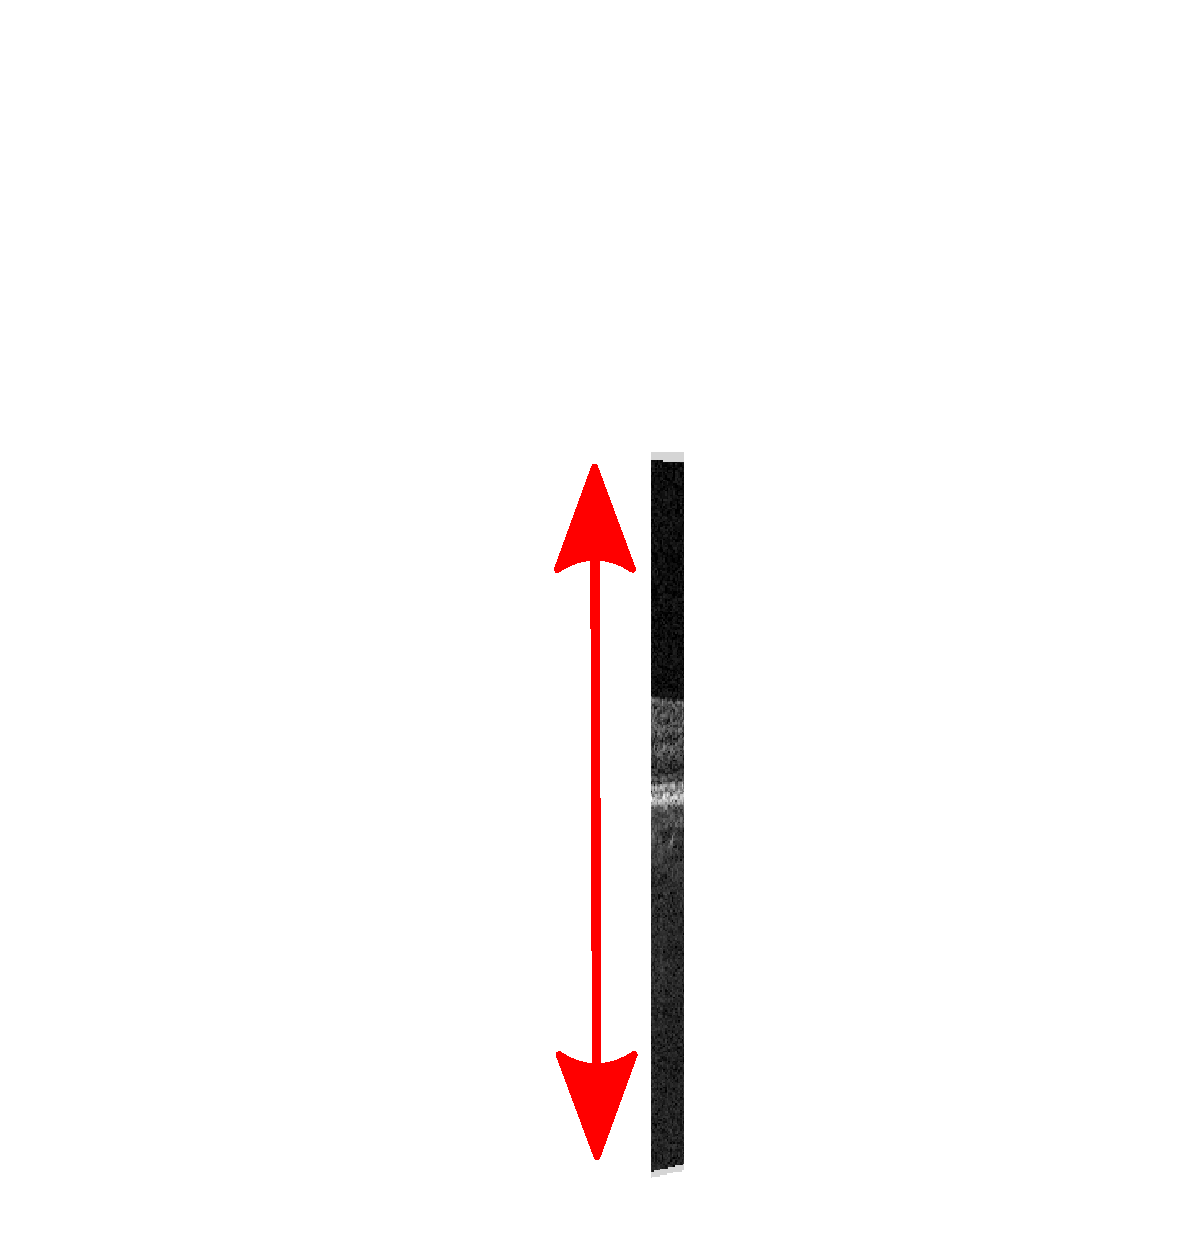
\includegraphics[height=0.5\textheight, trim={0cm  0 0 5cm},clip]{raster_scan_a.pdf}
                    \caption{Classical A-Scan}
                    \label{fig:}
                \end{figure}
            \end{column}\begin{column}{0.5\textwidth}
                \begin{figure}[]
                    \centering
                    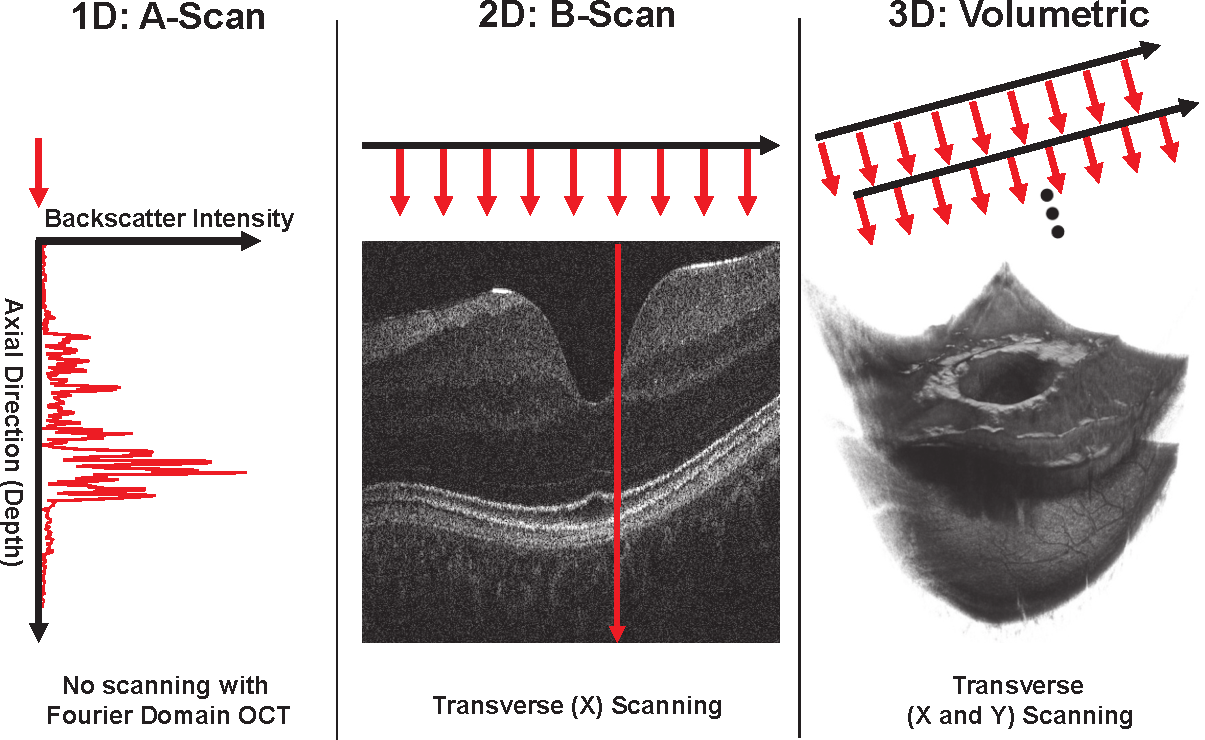
\includegraphics[height=0.5\textheight, trim={0  2cm 15cm 2cm},clip]{figures/OCTScanning.pdf}
                    \caption{No scanning with Fourier OCT}
                    \label{fig:}
                \end{figure}

            \end{column}
        \end{columns}
    }

\end{frame}

\begin{frame}
    \frametitle{OCT Scanning}
    \begin{itemize}
        \item 2D and 3D image construction by scanning the beam over the tissue while acquiring A-Scans
    \end{itemize}
    \begin{figure}
        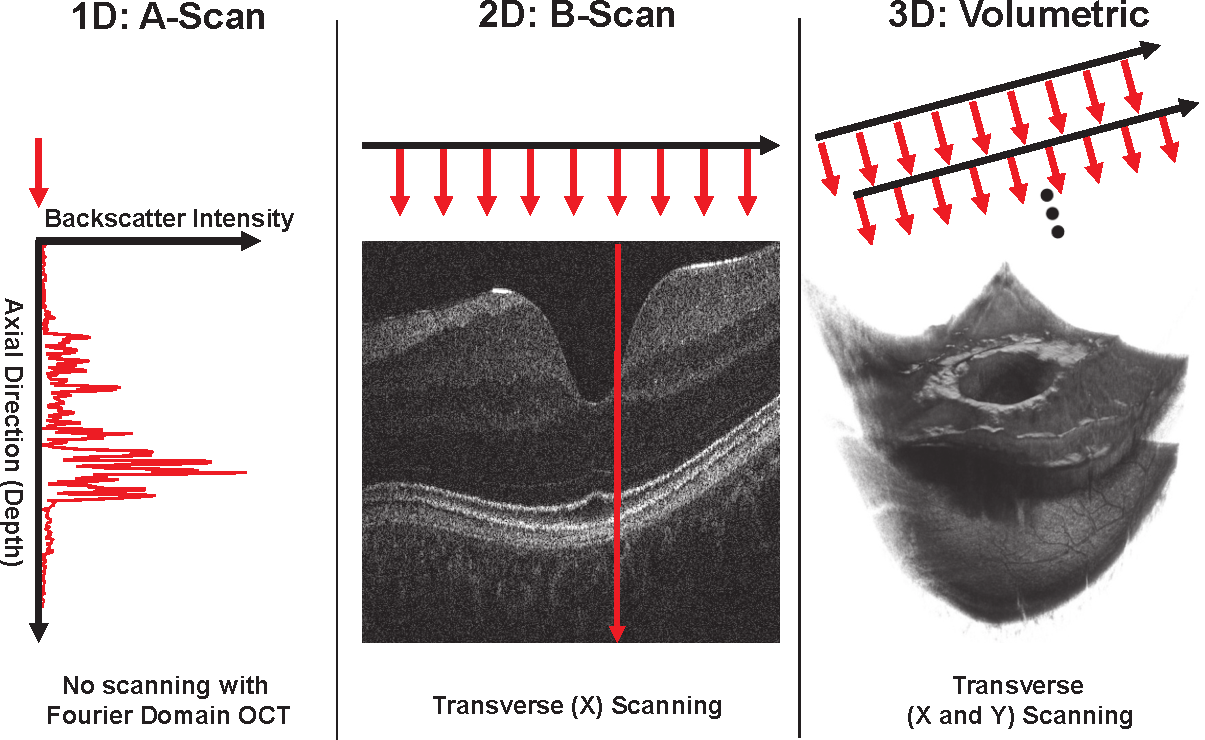
\includegraphics[height=0.65\textheight]{figures/OCTScanning.pdf}
        %	\caption{Interference Pattern for monochromatic light}
    \end{figure}

\end{frame}


\section{Applications}

\subsection{Ophthalmology}%
\label{sub:ophthalmology}

\begin{frame}\frametitle{Ophthalmology}
    \begin{itemize}
        \item Major tool in eye diagnostics and disease progression monitoring
        \item Age-related Macular Degeneration (AMD), Glaucoma, Diabetic Retinopathy
    \end{itemize}
    \begin{figure}
        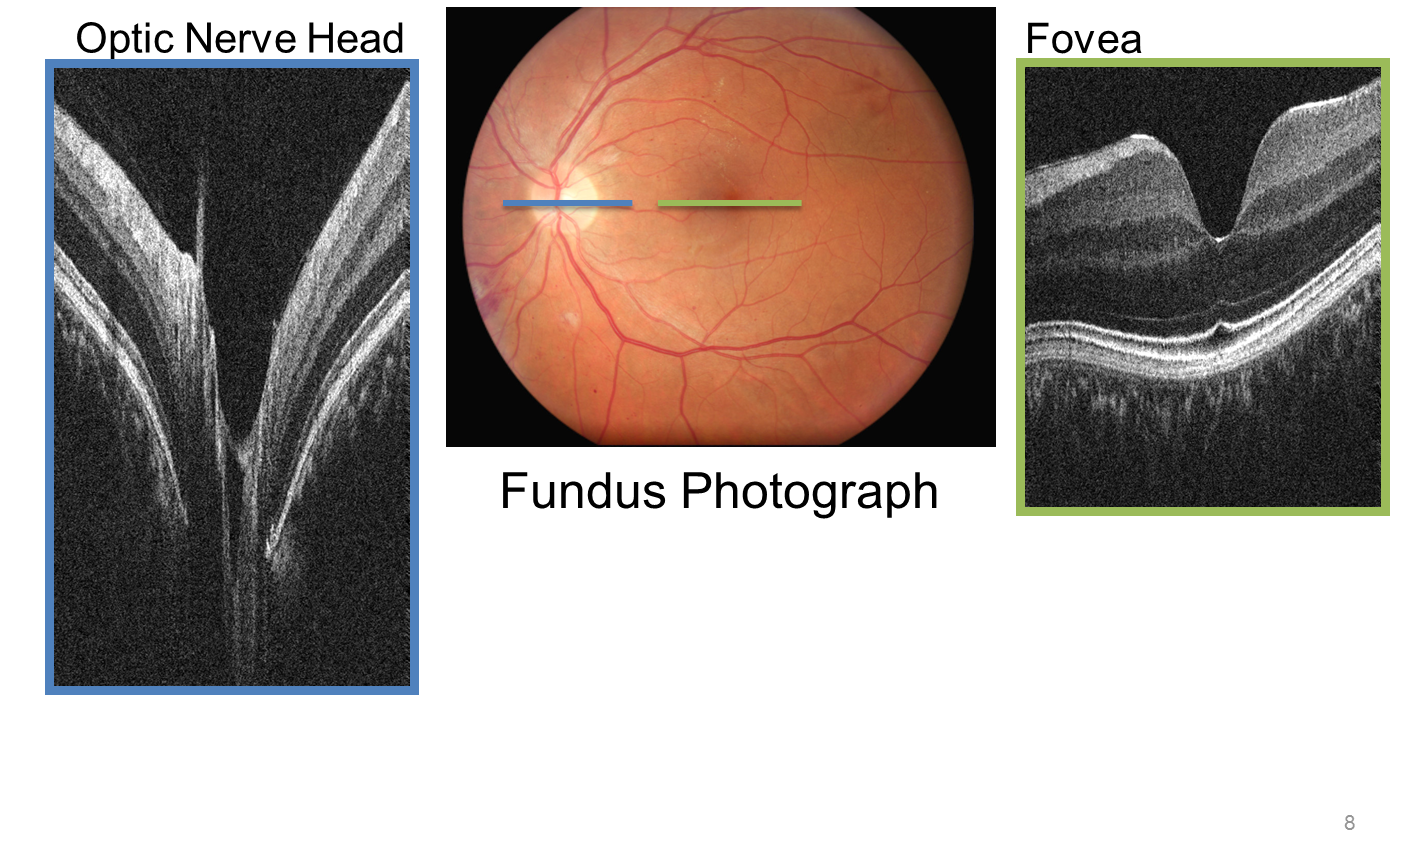
\includegraphics[height=0.85\textheight]{figures/FundusVsOCT.png}
        %	\caption{Interference Pattern for monochromatic light}
    \end{figure}

\end{frame}

\begin{frame}
    \frametitle{Example 2D Images}
    \begin{itemize}
        \item Normal subject vs. Age-related Macular Degeneration
        \item False Color
    \end{itemize}
    \begin{figure}
        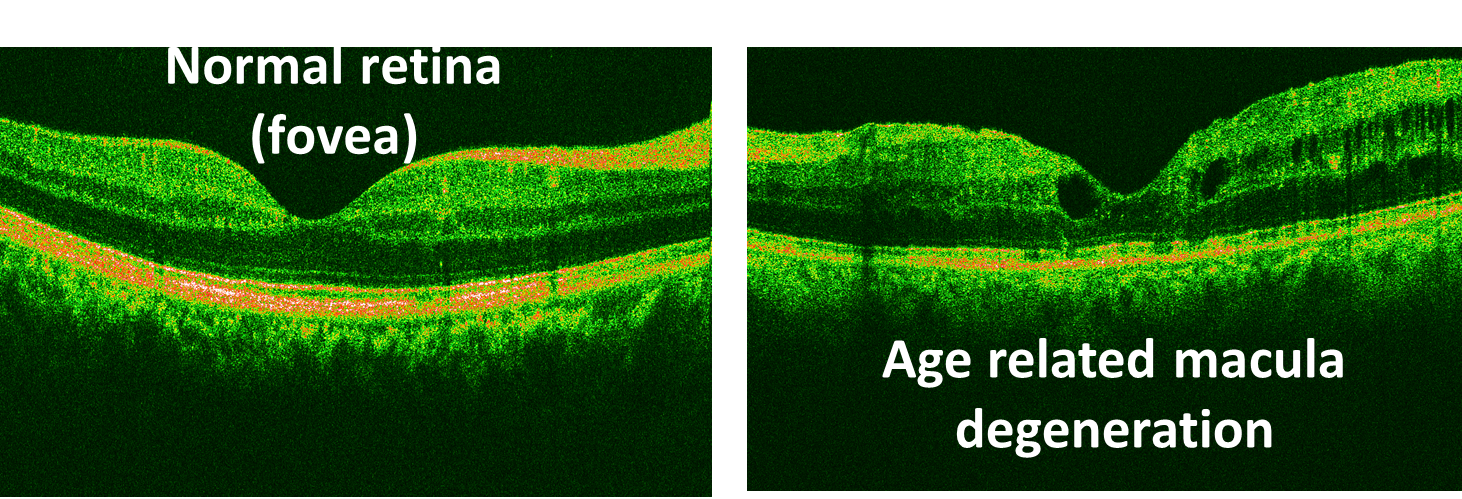
\includegraphics[width=\textwidth]{figures/NormalVSAMD.png}
        %	\caption{Interference Pattern for monochromatic light}
    \end{figure}

\end{frame}


\subsection{Cardiovascular Imaging}%
\label{sub:cardiovascular_imaging}


\begin{frame}
    \frametitle{Cardiovascular Imaging}
    \begin{itemize}
        \item OCT Probe in a catheder
        \item Blood is flushed out with transparent fluid to allow for optical imaging
        \item Allows the detection of plague, monitoring of stent placement etc.
    \end{itemize}

    \begin{figure}
        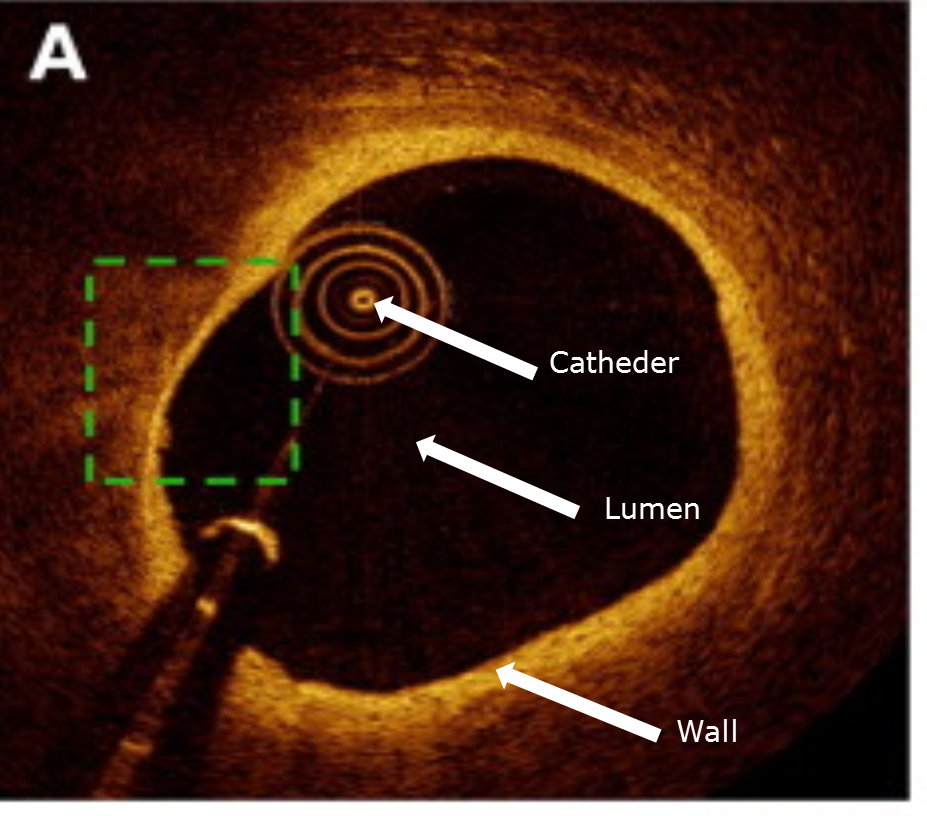
\includegraphics[height=0.55\textheight]{figures/Intravascular.png}
        \caption{J Am Coll Cardiol Intv. 2009;2(11):1035-1046. doi:10.1016/j.jcin.2009.06.019
        }
    \end{figure}
\end{frame}

\subsection{OCT Angiography}%
\label{sub:oct_angiography}

\begin{frame}{OCT Angiography}
    \vspace{-0.5cm}
    \begin{columns}[c, onlytextwidth]
        \begin{column}{0.5\textwidth}
            \begin{itemize}
                \item Contrast-agent-free vessel visualization
                \item Blood cells induce speckle noise
                \item Visualization of variance shows vessels
            \end{itemize}
        \end{column}\begin{column}{0.5\textwidth}
            \begin{figure}[tbp]
                \centering
                \newlength{\picwidth}
                \newlength{\picheight} % only for b-scans, en-face images are square and only use picwidth!
                \newlength{\mmwidth}
                \newlength{\mmheight}

                \setlength{\picwidth}{0.95\textwidth}
                \setlength{\picheight}{.866\picwidth} % factor = 433/500 (pixels height / pixels width)
                \setlength{\mmwidth}{0.0833\picwidth} % factor = 1mm / 3mm (3mm field size)
                \setlength{\mmheight}{0.513\picheight} % factor 1mm / (4.5um * 433) = 1mm / picheight, picheight = 4.5um axial pixel size * 433 pixels height

                \begin{tikzpicture}[outer sep=0,inner sep=0, scale=0.75]
                    % border lines are affected by clipping and thus only half as wide as specified
                    % this perfectly solves the issue that we need two lines next to each other inside the picture
                    \begin{scope}
                        \path[clip] (-.5\picwidth,.49\picwidth) -- (-.5\picwidth,-.2\picwidth) -- (.5\picwidth,.01\picwidth) -- (.5\picwidth,.49\picwidth) -- cycle;
                        \node{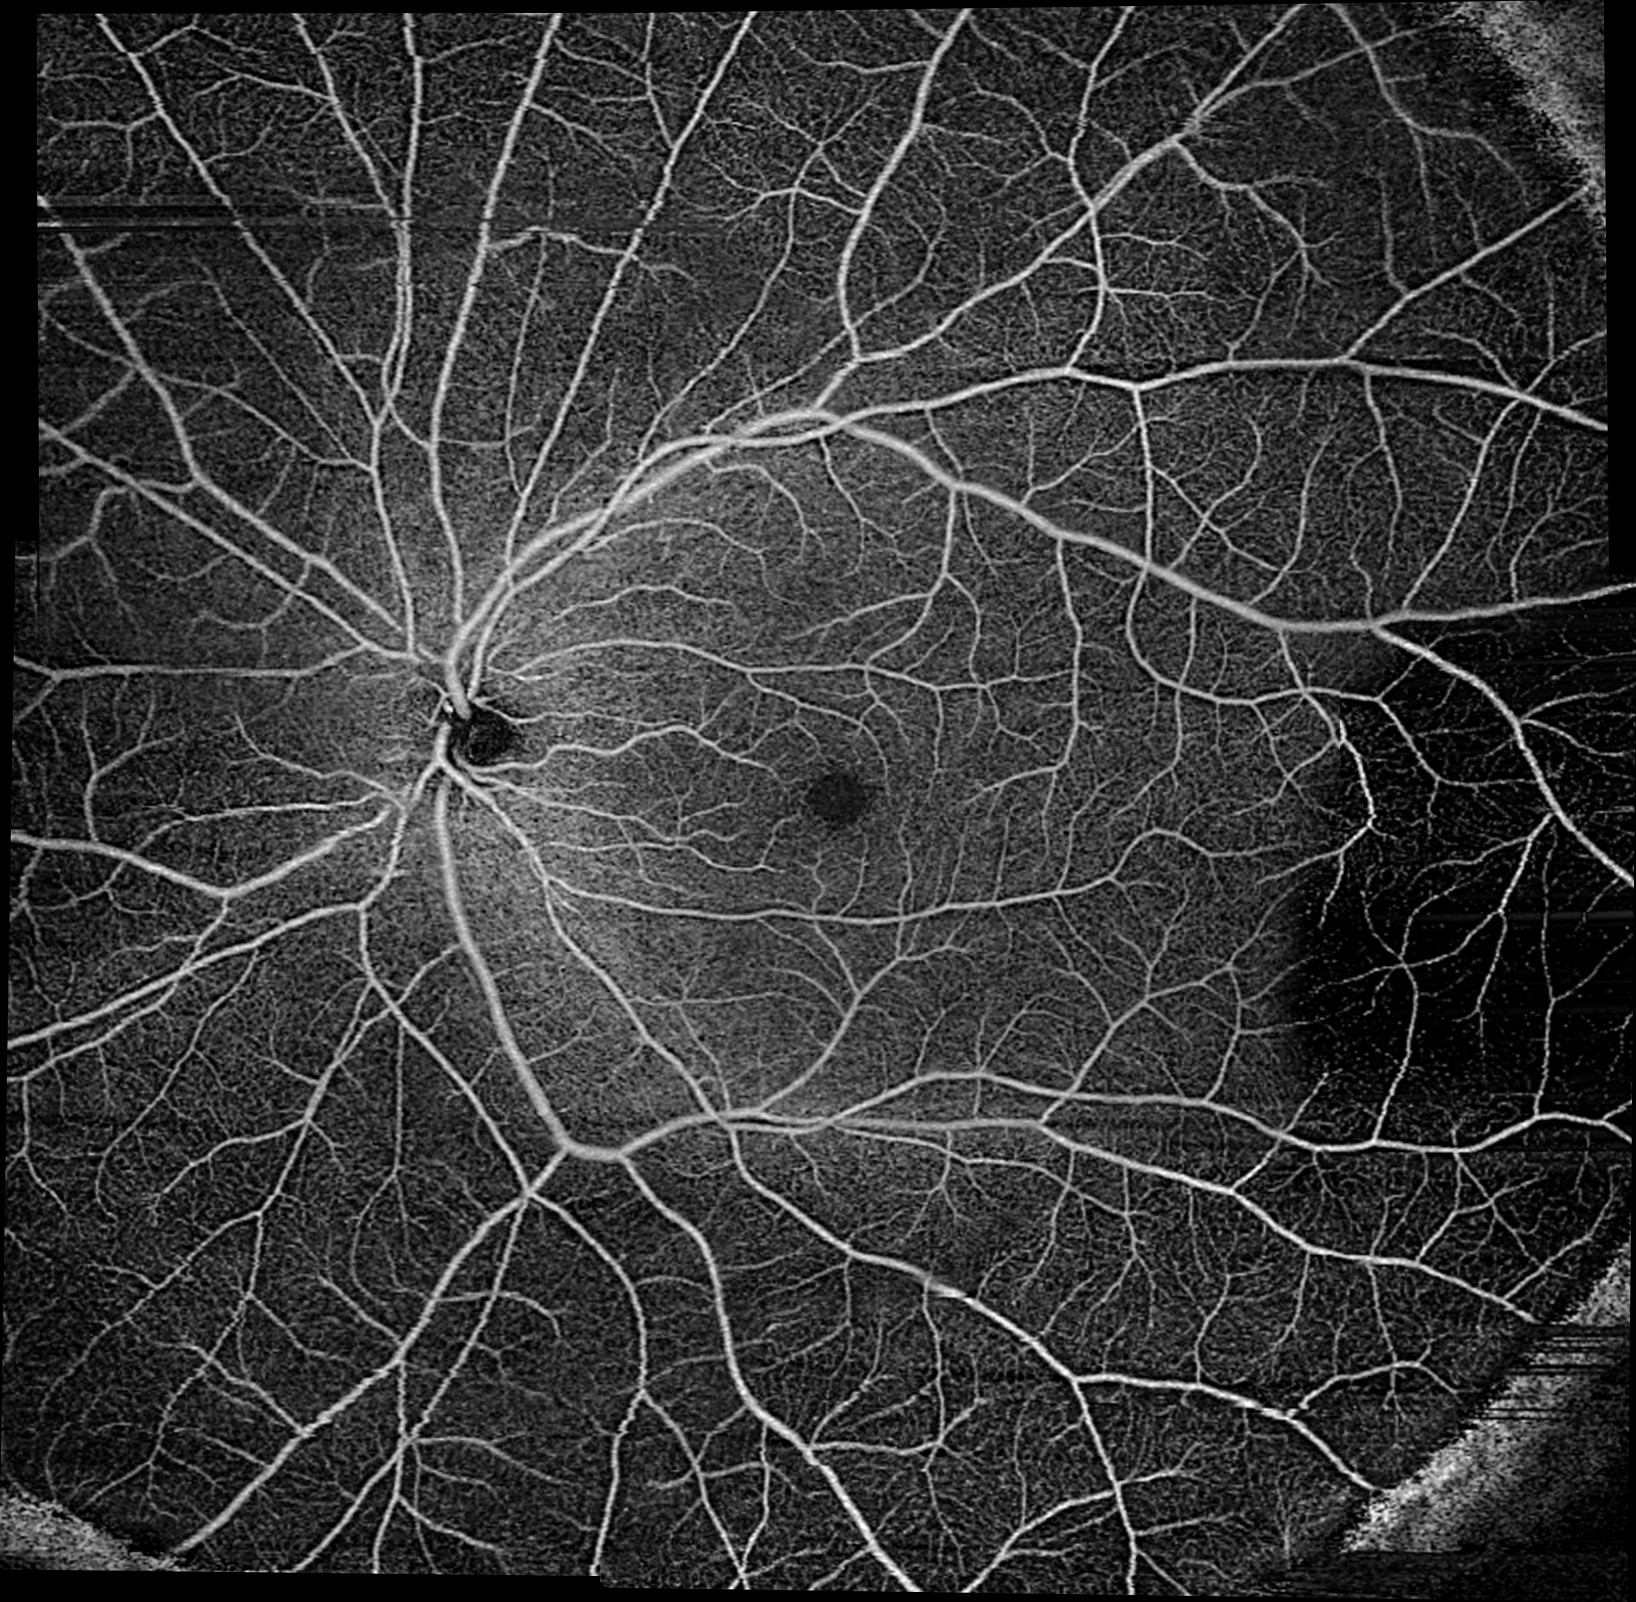
\includegraphics[width=\picwidth]{figures/Angiography_Superficial_Montage.png}};
                        \draw[color=red,ultra thick] (-.5\picwidth,.49\picwidth) -- (-.5\picwidth,-.2\picwidth) -- (.5\picwidth,.01\picwidth) -- (.5\picwidth,.49\picwidth) -- cycle;
                    \end{scope}
                    \begin{scope}
                        \path[clip] (-.5\picwidth,-.2\picwidth) -- (-.5\picwidth,-.49\picwidth) -- (.5\picwidth,-.2\picwidth) -- (.5\picwidth,.01\picwidth) -- cycle;
                        \node{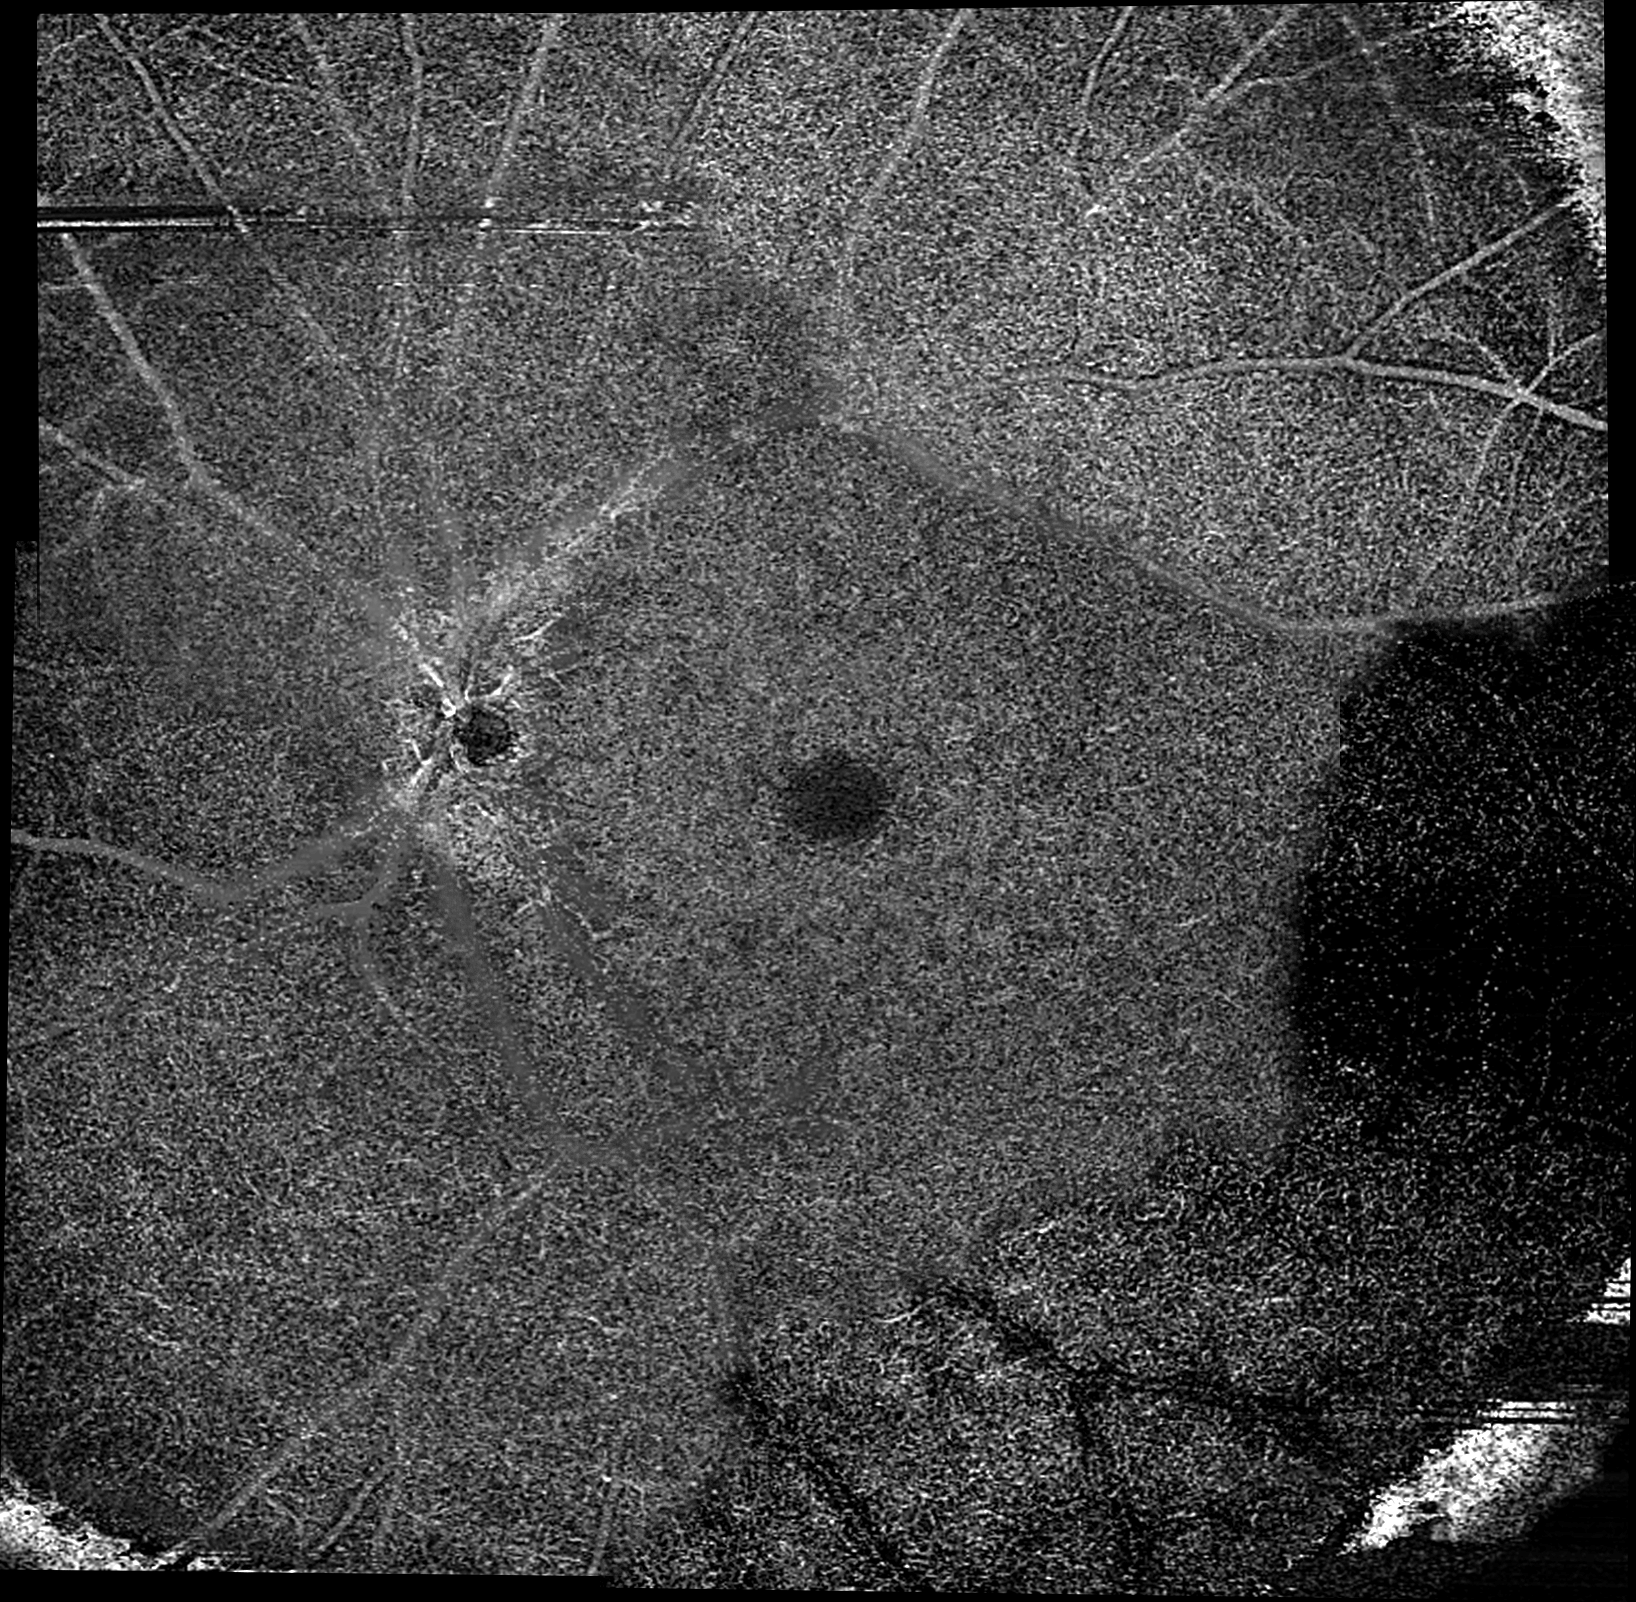
\includegraphics[width=\picwidth]{figures/Angiography_Deep_Montage.png}};
                        \draw[color=green,ultra thick,dashed] (-.5\picwidth,-.2\picwidth) -- (-.5\picwidth,-.49\picwidth) -- (.5\picwidth,-.2\picwidth) -- (.5\picwidth,.01\picwidth) -- cycle;
                    \end{scope}
                    \begin{scope}
                        \path[clip] (.5\picwidth,-.49\picwidth) -- (.5\picwidth,-.2\picwidth) -- (-.5\picwidth,-.49\picwidth) -- cycle;
                        \node{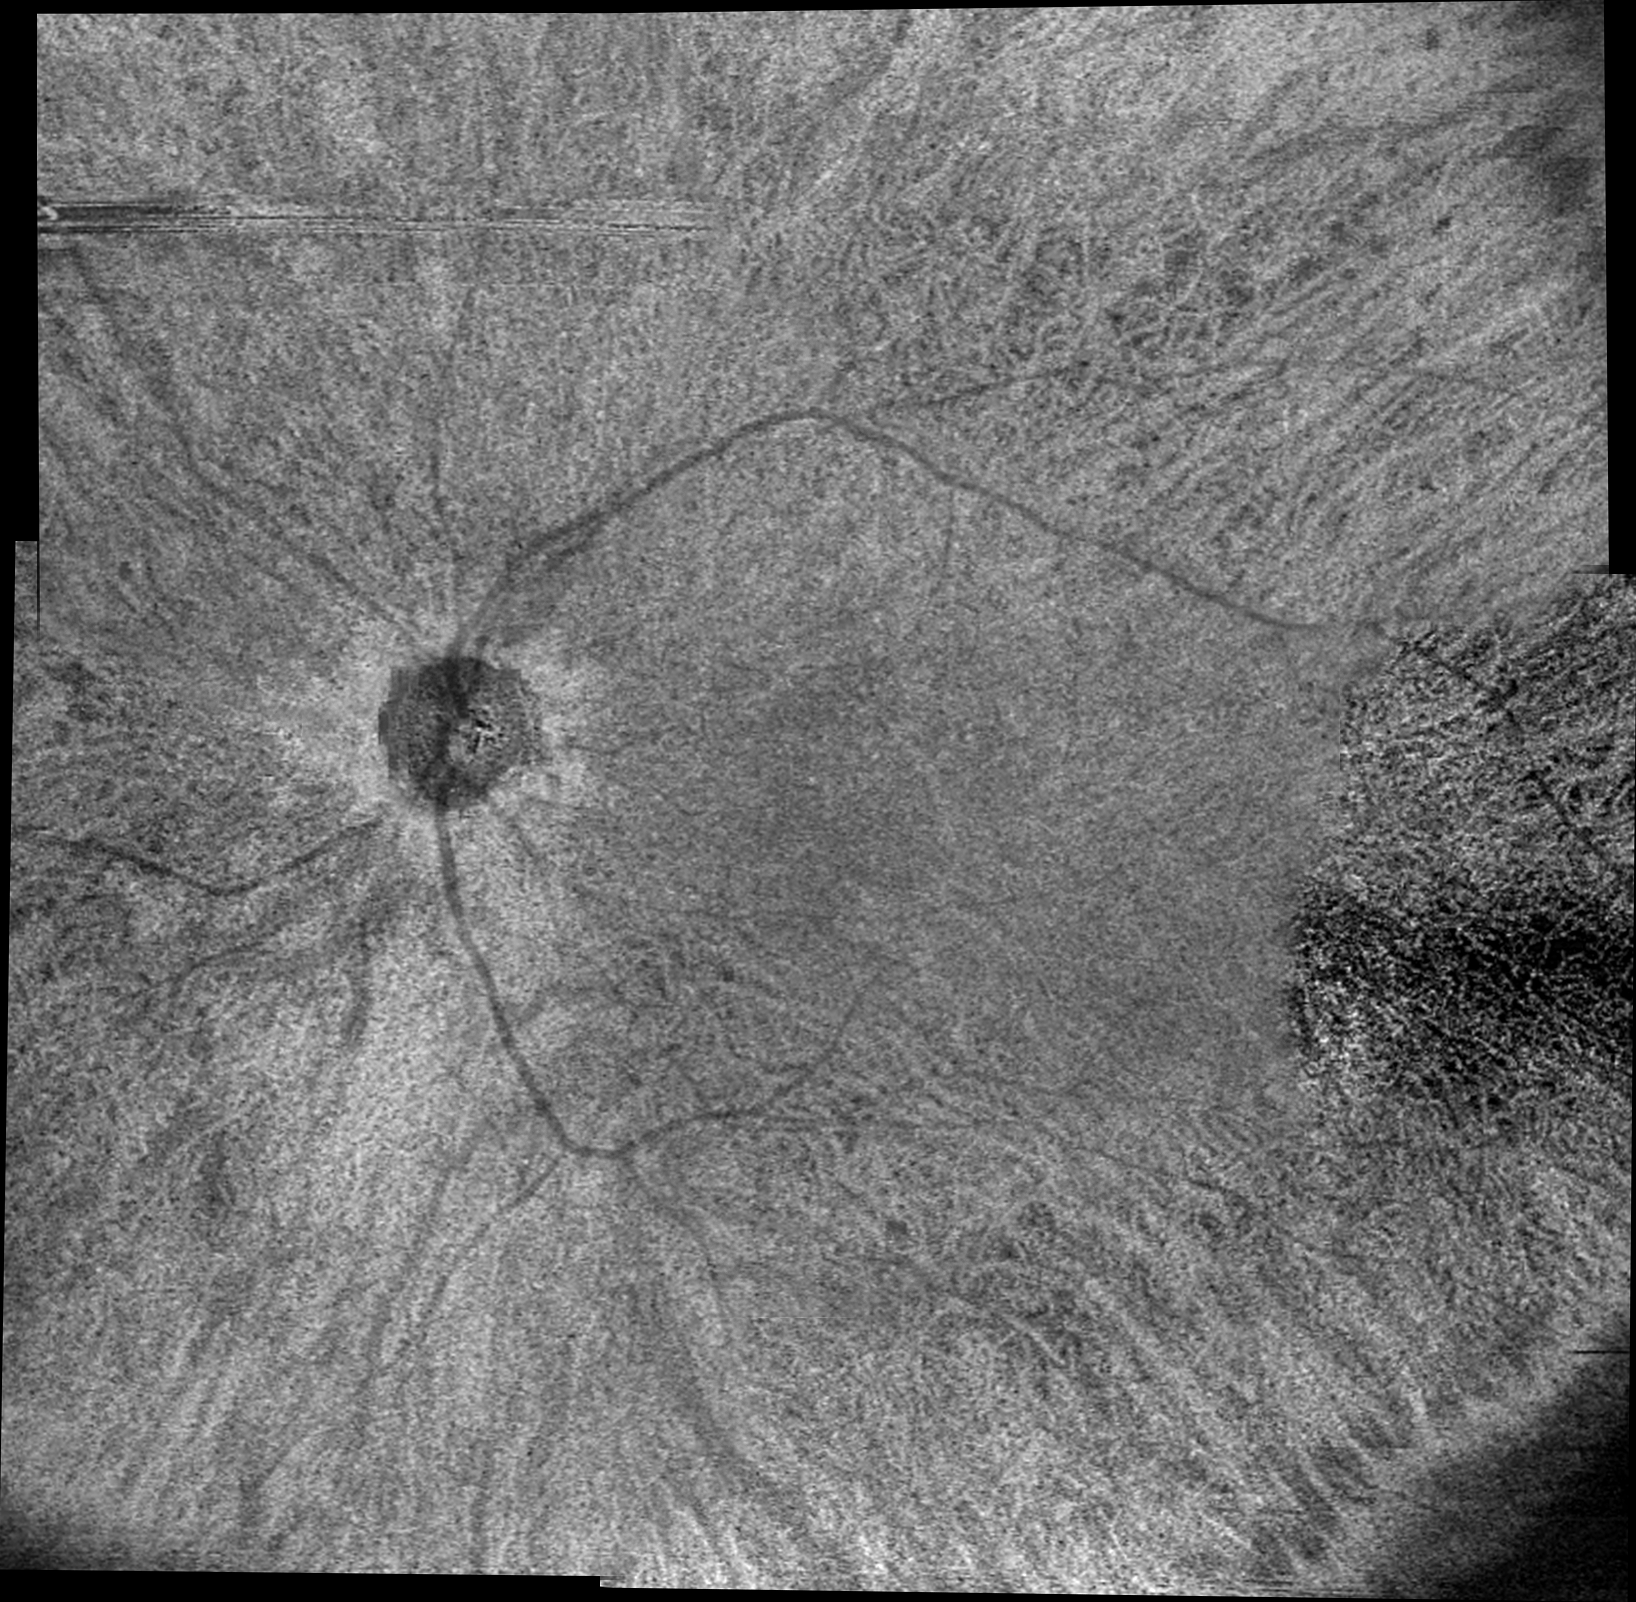
\includegraphics[width=\picwidth]{figures/Angiography_Choroid_Montage.png}};
                        \draw[color=blue,ultra thick,dotted] (.5\picwidth,-.49\picwidth) -- (.5\picwidth,-.2\picwidth) -- (-.5\picwidth,-.49\picwidth) -- cycle;
                    \end{scope}
                    \draw[color=white,ultra thick] (-.42\picwidth,-.42\picwidth+\mmwidth) -- ++(0,-\mmwidth) -- ++(\mmwidth,0);
                    \node[rotate=-90,anchor=north,color=white,inner sep=0.7mm] at (-.42\picwidth,-.42\picwidth+\mmwidth/2) {\tiny 1mm};
                    \node[anchor=north,color=white,inner sep=0.7mm] at (-.42\picwidth+\mmwidth/2,-.42\picwidth) {\tiny 1mm};
                \end{tikzpicture}
                \caption{3-D OCT angiography results in a layered reconstruction of the vessels for each retinal layer. Here we show a wide 12 mm $\times$ 12 mm field of view of the superficial and deep retina as well as the choroid (from top to bottom).}
                \label{fig:oct_acta}
            \end{figure}
        \end{column}
    \end{columns}

    %
\end{frame}


\section{Conclusion}

\begin{frame}[c]{Take Home Messages}
    \begin{itemize}
        \setlength\itemsep{0.3cm}
        \item<2-> Optical Coherence Tomography: In situ imaging
        \item<3-> High resolution, non-invasive
        \item<4-> Key concepts:
              \begin{itemize}
                  \item Light as a wave
                  \item Interference
                  \item Coherence length
              \end{itemize}
        \item<5-> Standard in Ophthalmology
    \end{itemize}
\end{frame}


\begin{frame}
    \frametitle{Further Reading}
    \begin{itemize}
        \setlength\itemsep{0.2cm}
        \item \fullcite{husvogt18}
        \item Wolfgang Drexler, James G. Fujimoto  : ``Optical Coherence Tomography: Technology and Applications'', Springer, 2008
        \item Mark E. Brezinski: ``Optical coherence tomography: principles and applications'', Elsevier, Oxford, 2006

    \end{itemize}
\end{frame}


\end{document}
